\subsection{Resultados de la Extracción de Características}

En esta sección se presentan los resultados obtenidos de la extracción de características de las \glspl{url} analizadas. La extracción de características es un paso fundamental en el proceso de creación del modelo de detección de \gls{phishing} y otras amenazas web, ya que permite transformar las \glspl{url} en un conjunto de datos estructurados que pueden ser utilizados por los algoritmos de \textit{machine learning} para el entrenamiento y la predicción.

\subsubsection*{Estadísticas Descriptivas}

Las características extraídas y sus respectivas estadísticas descriptivas se resumen en los siguientes puntos:

\begin{itemize}
    \item \textbf{Longitud de la \gls{url}}: 
    La longitud de las \glspl{url} analizadas presenta una media que indica que la mayoría de las \glspl{url} son relativamente cortas, concentrándose entre 10 y 50 caracteres. Esto sugiere que las \glspl{url} en general tienden a ser más concisas.

    \item \textbf{Cantidad de Dígitos en la \gls{url}}: 
    La cantidad de dígitos en las \glspl{url} muestra una distribución sesgada hacia la izquierda, con la mayoría de las \glspl{url} conteniendo pocos dígitos. Esto puede estar relacionado con el intento de los atacantes de hacer las \glspl{url} más legítimas.

    \item \textbf{Cantidad de Letras en la \gls{url}}: 
    La distribución de la cantidad de letras en las \glspl{url} también está sesgada hacia la izquierda, indicando que la mayoría de las \glspl{url} contienen una cantidad moderada de letras, lo que puede ayudar a evitar la detección por parte de los usuarios.

    \item \textbf{Cantidad de Caracteres Especiales en la \gls{url}}: 
    Los caracteres especiales como puntos, guiones y guiones bajos son relativamente pocos en la mayoría de las \glspl{url}. Esto sugiere que las \glspl{url} maliciosas intentan mantener una apariencia simple para evitar la detección.

    \item \textbf{Longitud del Dominio}: 
    La longitud de los dominios en las \glspl{url} analizadas varía, pero la mayoría son relativamente cortos. Esto podría deberse a que los dominios más cortos son más fáciles de recordar y parecen más legítimos.

    \item \textbf{Cantidad de Vocales en el Dominio}: 
    La cantidad de vocales en el dominio varía considerablemente, lo que puede indicar que los atacantes utilizan una mezcla de nombres de dominio complejos y simples para evitar la detección.

    \item \textbf{Longitud del Directorio}: 
    La longitud del directorio en las \glspl{url} muestra una distribución sesgada hacia la izquierda, indicando que la mayoría de los directorios son cortos. Esto sugiere que las \glspl{url} maliciosas tienden a no profundizar en la estructura del sitio.

    \item \textbf{Número de Parámetros}: 
    La mayoría de las \glspl{url} tienen pocos parámetros, lo que sugiere que los atacantes prefieren mantener las \glspl{url} simples y fáciles de manejar.

    \item \textbf{Número de Subdominios}: 
    La cantidad de subdominios en las \glspl{url} es generalmente baja, lo que indica que los atacantes no suelen utilizar estructuras de dominio complejas.

    \item \textbf{Entropía del \gls{sld}}: 
    La entropía del \gls{sld} varía significativamente entre las \glspl{url}, lo que sugiere una diversidad en la complejidad de los nombres de los dominios utilizados en las \glspl{url} maliciosas.

    \item \textbf{Edad del Dominio (días)}: 
    La edad de los dominios varía ampliamente, con algunos dominios muy antiguos y otros muy recientes. Esto puede indicar que los atacantes utilizan tanto dominios nuevos como antiguos para sus ataques.

    \item \textbf{Tiempo Restante para la Expiración (días)}: 
    Similar a la edad del dominio, el tiempo restante para la expiración también varía ampliamente, lo que sugiere que los atacantes no tienen una preferencia clara en cuanto al tiempo de vida restante de un dominio.
\end{itemize}

\subsubsection*{Distribuciones de Características}

Las distribuciones de las características principales se representan en los siguientes histogramas:

\begin{figure}[H]
    \centering
    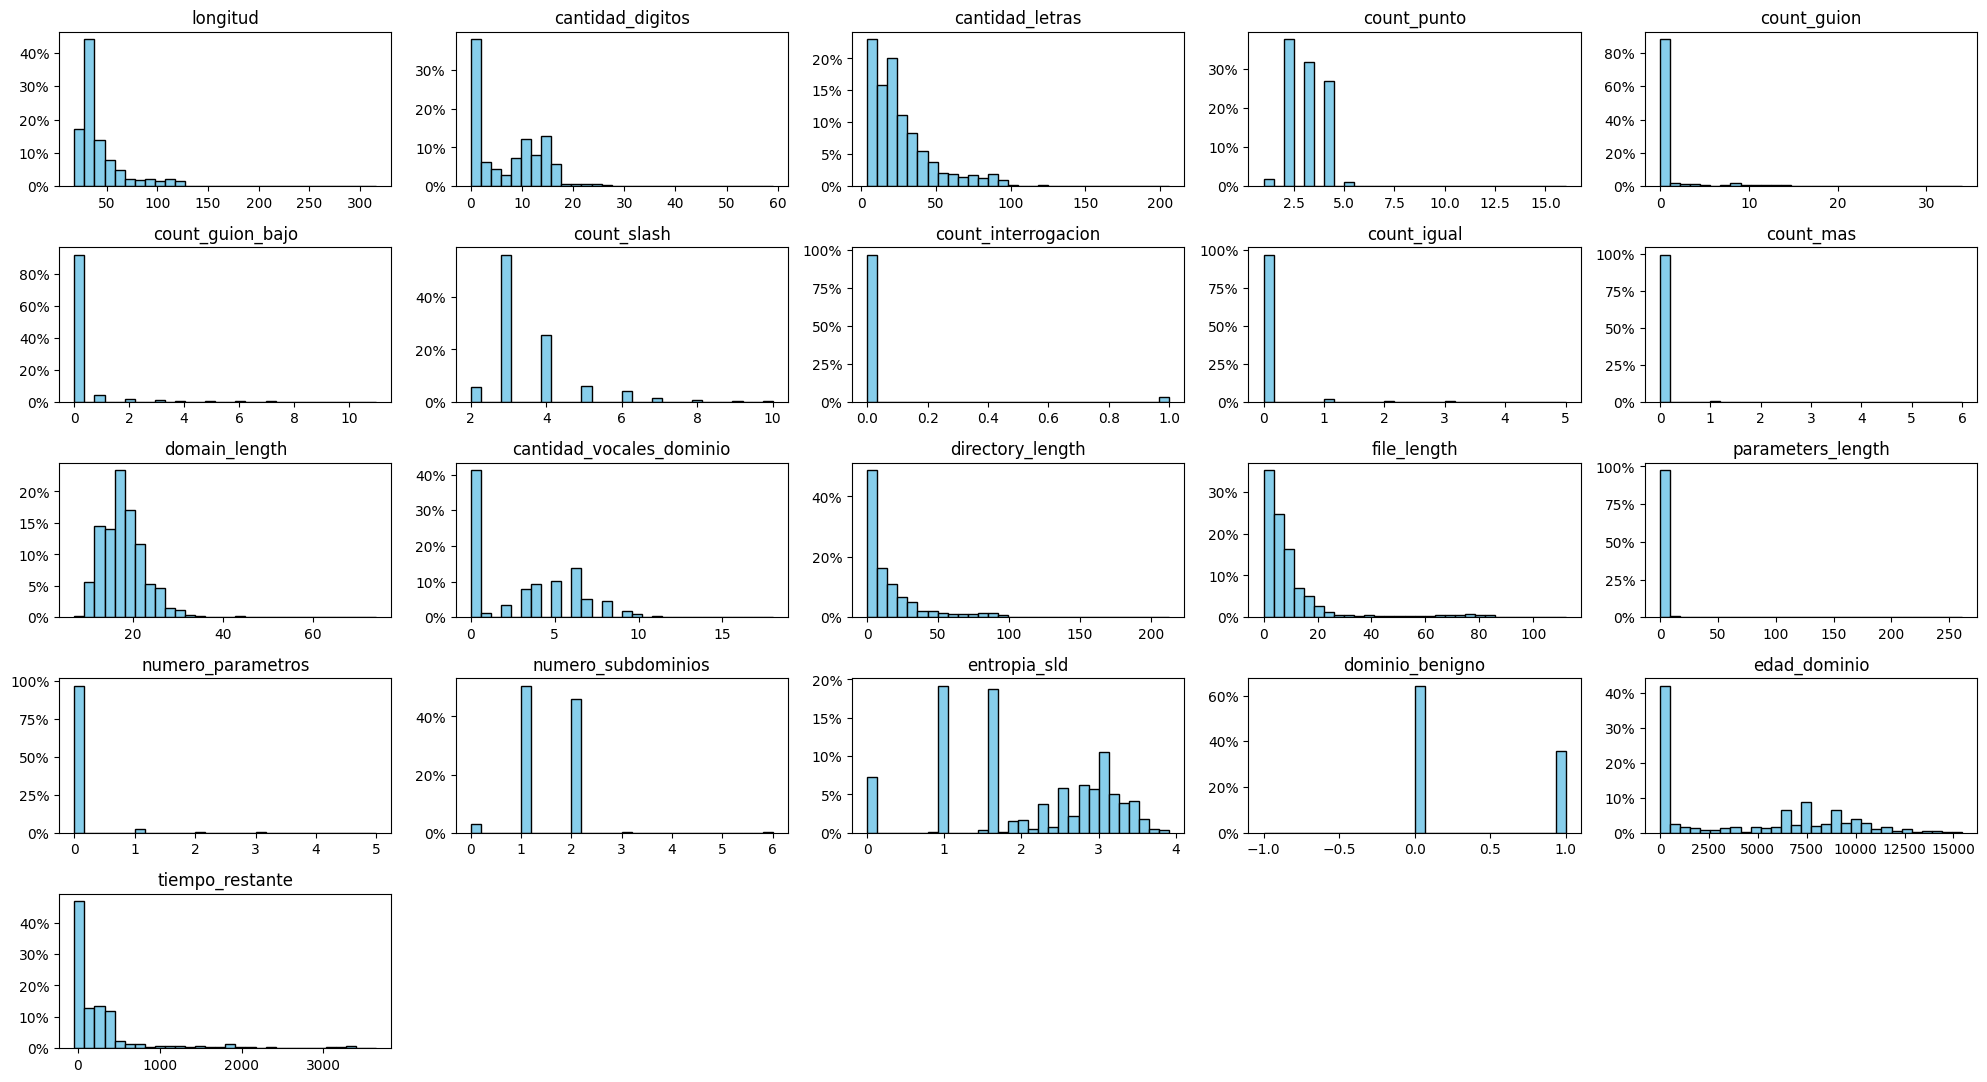
\includegraphics[width=\textwidth]{histogram1.png}
    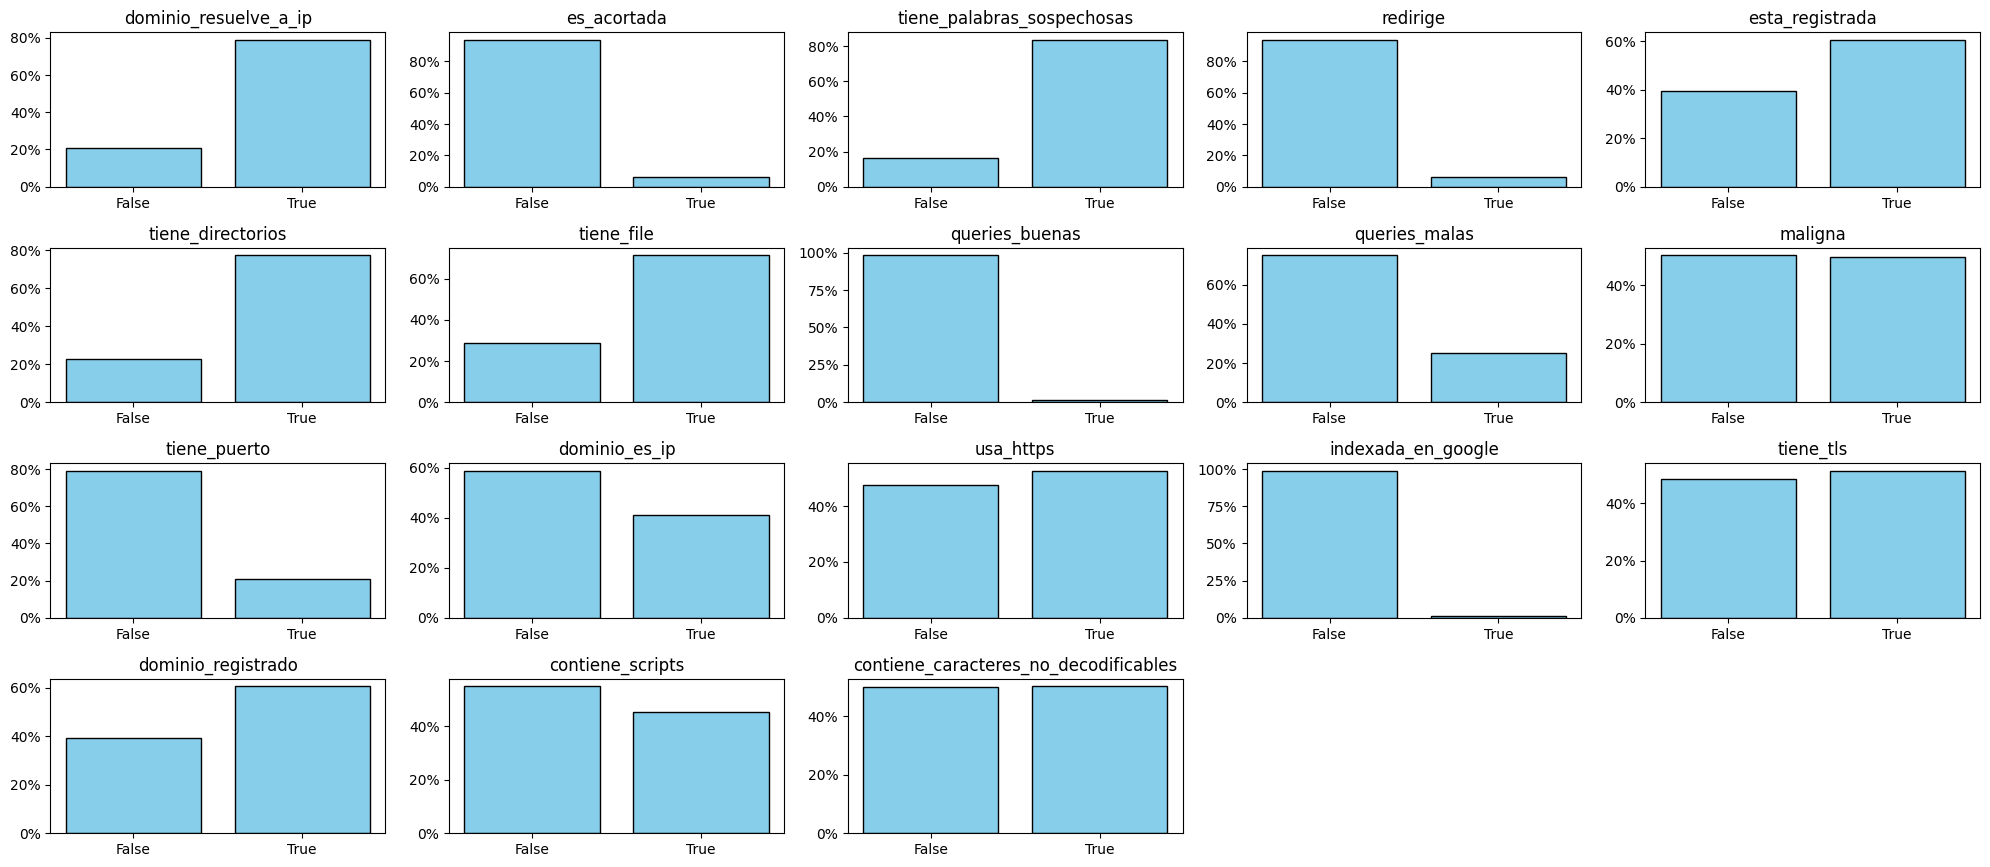
\includegraphics[width=\textwidth]{histogram2.png}
    \caption{Distribuciones de las características principales de las \glspl{url}.}
    \label{fig:histograms}
\end{figure}

\subsubsection*{Análisis de Correlación}

El análisis de correlación entre las características revela relaciones interesantes:

\begin{itemize}
    \item \textbf{Correlaciones Altas}: 
    Se observan correlaciones significativas entre características como si la \gls{url} esta registrada, la cantidad de letras y el uso de \gls{https}. Esto puede indicar que las \glspl{url} más largas y con más letras tienden a usar \gls{https}, lo cual puede estar relacionado con la seguridad de la \gls{url}.

    \item \textbf{Redundancia de Características}: 
    Algunas características muestran una alta correlación, lo que sugiere redundancia. Por ejemplo, la característica de uso de \gls{https} está altamente correlacionada con la longitud de la \gls{url} y la cantidad de letras, lo que llevó a la decisión de eliminar estas características en algunos modelos para evitar la multicolinealidad.
\end{itemize}

\begin{figure}[H]
    \centering
    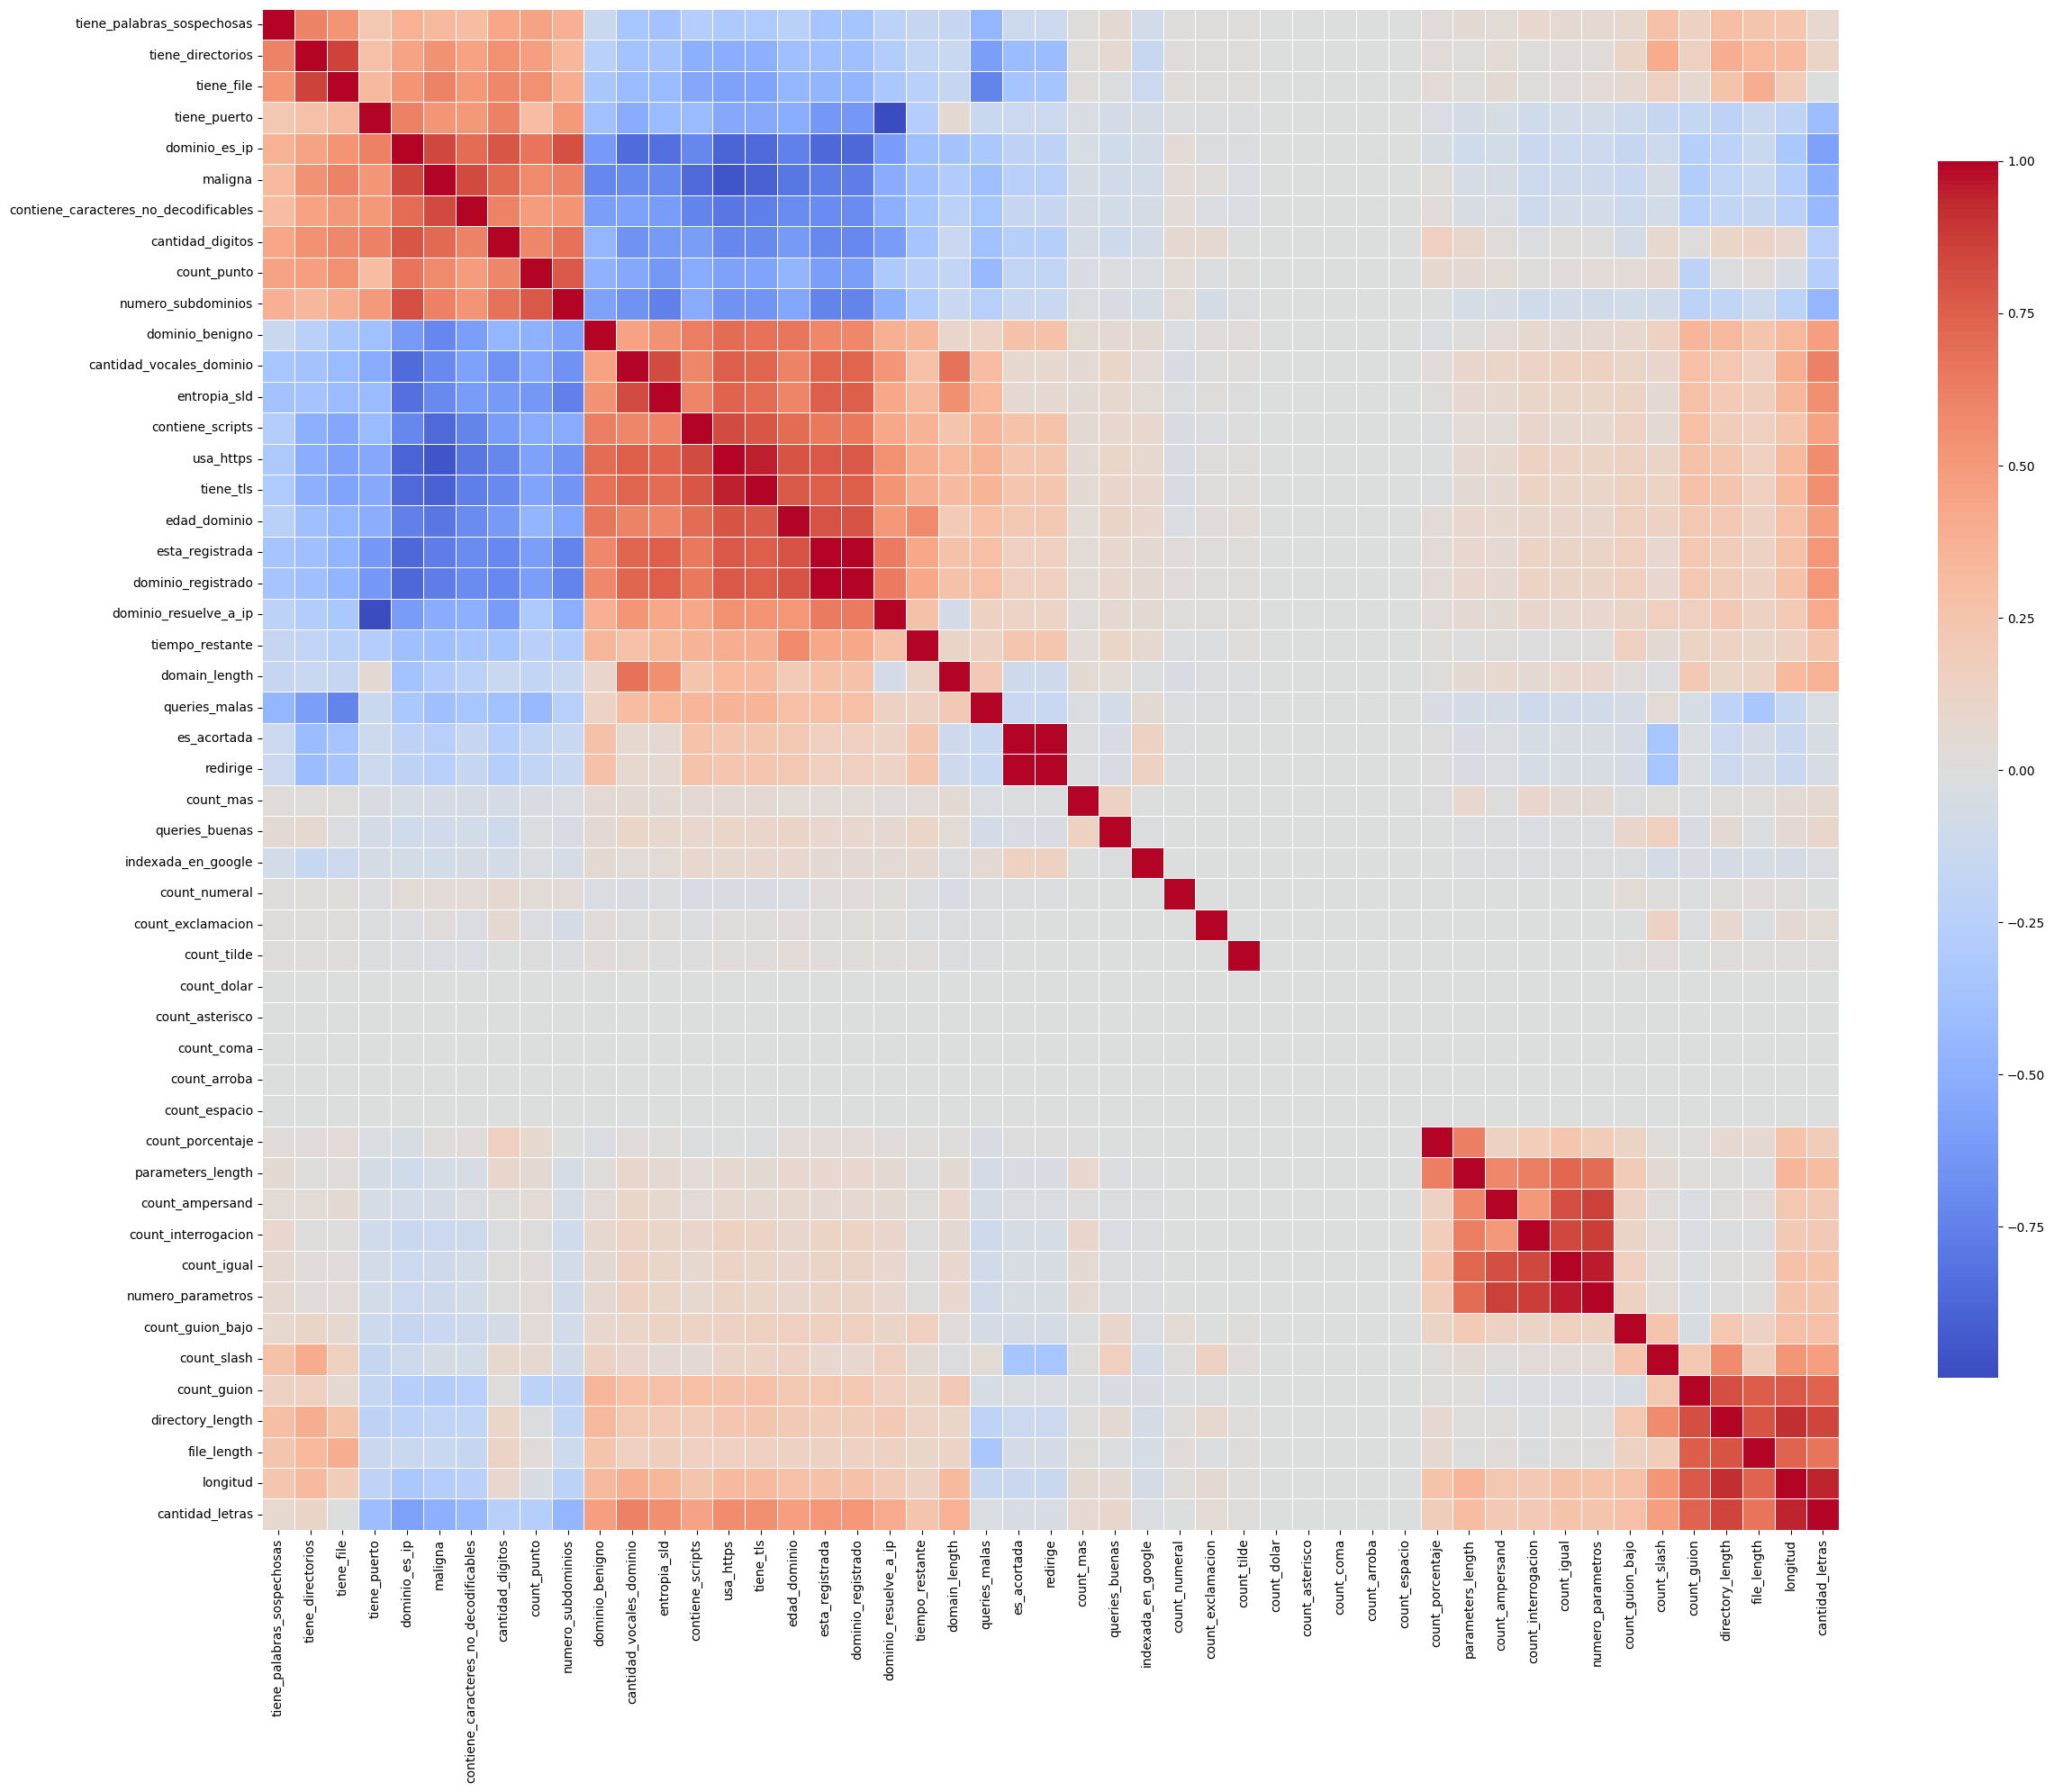
\includegraphics[width=\textwidth]{heatmap.png}
    \caption{Mapa de correlación entre las características extraídas de las \glspl{url}.}
    \label{fig:correlation_matrix}
\end{figure}











